%%=================== Compiler Directives =================%%
%%                                                         %%
% !TeX program = pdflatex
% !TeX encoding = utf8
% !BIB TS-program =bibtex8
%%                                                         %%
%%=========================================================%%



%%==================================================================================%%
%%                                                                                  %%
%%  сайт конференції conf.ipt.kpi.ua				                                %%
%%  проект на ShareLaTeX https://ru.sharelatex.com/project/56e308d7bad2a71c56327601 %%
%%  проект на OverLeaf https://www.overleaf.com/read/ckvrdbwwkzng                   %%
%%                                                                                  %%
%%==================================================================================%%



%%===================== Class Options =====================%%
%%                                                         %%
%%                                                         %%
				\documentclass{ConfFTI}
%%                                                         %%
%%   incollection  - create black footers and headers 	   %%
%%   alone 		   - create pagenumber in footers          %%
%%=========================================================%%



%%===================== Package Placing ===================%%

\usepackage[most]{tcolorbox}
\usepackage{makecell}
\usepackage{booktabs}
\usepackage{tabularx}
\usepackage{mathtools}
\usepackage{dsfont}
\usepackage{mathrsfs}
\usepackage{wrapfig}
\usepackage{subfig}
\usepackage{bbm}
%==== Пакет для запису хімічних формул =====
\usepackage[version=4]{mhchem}
%==== Пакет для створення діаграм та графіків =====
\usepackage{forest}
\usepackage{tikz}
\usepackage{pgfplots}
\usetikzlibrary{shadows,arrows.meta}

%%================== Команди користувача ==================%%
%%            Тут можна визначити власні команди           %%
\def\templateurl{%
\href{https://drive.google.com/file/d/0B_zxNbdfIopVUjVjeTJGb05mdjQ/view}%
{\texttt{\jobname.zip}}}
%%=========================================================%%




%%======================= Назва тез =======================%%
%%                                                         %%
%%                                                         %%
\title{Предварительная сегментация изображения для ускорения алгоритмов стереозрения}
%%                                                         %%
%%                                                         %%
%%=========================================================%%



%%======================== AUTHORS ========================%%
%%  Якщо бажаєте, введіть e-mail автора в квадратних дужках:
\author{О.~А.~Лавягина}{1} % Команда \email --- вставляє значення наведене в реєстраційній формі

\author{Е.~В.~Водолазский}{2}

%\author{А.~В.~Третій}{2}

%% Якщо  автор працює в кількох установах, то треба вводити номери установ через кому, наприклад так:
%\author[email3@mail.com]{А.~В.~Четвертий}{1,2}

%% значки "~" біля ініціалів і прізвищ означають нерозривний пробіл.



%%========= Назви установ, в яких працюють автори ==========%%

\affiliation{\ntuuipt}{1}
%% Тут введіть установув якій працює, або навчається перший автор.
%% Введіть \ntuu якщо автор навчається, або працює в НТУУ "КПІ"
%% Введіть \ntuuipt якщо автор навчається, або працює в Фізико-технічному інституті
\affiliation{Международный научно-учебный центр информационных технологий и систем \\
             НАН Украины и МОН Украины}{2}
%% Тут введіть установу в якій працює, або навчається другий автор



%%================== Реєстраційна форма ===================%%
%%                                                         %%
%%                                                         %%
\FullName{Лавягіна Ольга Олексіївна}                       % Повне ім'я доповідача (перший автор)
\Birthday{25.03.1997}                                      %% Дата народження доповідача
\Position{студент}                                         %% Посада доповідача
\phone{+380995237872}                                      %% Телефонний номер доповідача
\authoremail{olya.lavyagina@gmail.com}                     %% Email доповідача
\confsection{Математичне та комп’ютерне моделювання}       %% Секція конференції, на яку подається доповідь
\copynum{1}                                                %% Кількість копій збірника матеріалів, необхідних автору
\NeedLiving{Ні}                                            %% Потреба в житлі (Ні/Хостел/Готель/інше)
\NeedInvitation{Ні}                                        %% Чи потрібне запрошення на конференцію?
%%                                                         %%
%%                                                         %%
%%=========================================================%%



%%============ Тут вводьте номери PACS або УДК ============%%
%%                                                         %%
%\pacs{ }
\udc{004.93.11}
%%                                                         %%
%%=========================================================%%



%%============= Тут заповніть ключові слова ===============%%
\keywords{бинокулярное стереозрение, алгоритм диффузии, сегментация, карта глубин, трёхмерная модель}
\abstract{%
	 % Замість тексту, наведеного нижче, введіть текст анотації
	 Одной из актуальных проблем компьютерного зрения является
	 задача бинокулярного стереозрения.
     В данной работе приводится постановка
     задачи стереозрения по двум выровненным изображениям
     одного объекта или поверхности, алгоритм диффузии для решения этой задачи,
     а также предлагается метод ускорения этого алгоритма с помощью
     предварительной сегментации изображения.
}


%%====================================================================================%%
\begin{document}



%%=========Замість слова ukrainian (russian, english) введіть мову ваших тез =========%%
%%                                                                                    %%
\PaperLanguage{russian} %
%%                                                                                    %%
%%====================================================================================%%


%%====================================================================================%%
\section*{Введение}
%%====================================================================================%%

В основе получения трёхмерной
модели объекта или поверхности
лежит построение карты глубин с помощью решения задачи стереозрения.
Для этого используются различные алгоритмы,
среди которых алгоритм диффузии, который хорошо справляется с задачей,
но работает достаточно медленно.
В данной работе предложен способ ускорения алгоритма диффузии
для решения задачи стереозрения с помощью
предварительной сегментации изображения.

%%====================================================================================%%
\section{Постановка задачи}
%%====================================================================================%%

Дано левое полутоновое изображение $L \; : \; T \to C$
и правое полутоновое изображение $R \; : \; T \to C$,
где
$T = \left\{
    \left(x, y \right) \; \middle| \;
    1 \le x \le w, \,
    1 \le y \le h
\right\}$~--~множество координат пикселей изображения,
$w$~--~ширина изображения, $h$~--~высота изображения,
а $C= \left\{ 0, \dotsc, 255 \right\}$~--~множество интенсивностей пикселей.

Два изображения получаются за счёт сдвига камеры.
В связи с этим наблюдается параллакс~--~проекции
объектов на изображение двигаются.
Считаем, что камера перемещается ровно вбок.
Это значит,
что проекции объектов на изображение тоже перемещаются исключительно вбок.
Строим такую модель, согласно которой объекты не перекрываются друг другом.
Это не ограничивает её область применения,
и алгоритм можно использовать для перекрывающихся объектов,
что видно из экспериментов.

Таким образом, строка с вертикальной координатой $y$
на левом изображении соответствует
строке с вертикальной координатой $y$ на правом изображении.
Горизонтальная координата $x$ каждого пикселя левого изображения
$\left( x, y \right) \in T$
сдвигается влево на величину $d \left( x, y \right)$
для получения координаты соответствующего пикселя на правом изображении
$\left( x - d \left( x, y \right), y \right)$.
Множество всех возможных сдвигов горизонтальной координаты пикселя
равно $D = \left\{ 0, \dotsc, M \right\}$,
где $M$~--~фиксированный максимальный сдвиг.

Строится $\left| T \right|$-дольный граф-решётка,
в котором каждой доле соответствует один пиксель
(рис.~\ref{fig:grid:graph:pixels}).
Будем называть доли графа объектами.
Каждый объект $\left( x, y \right) \in T$ имеет $\left| D \right|$ вершин
$\left(x, y , d \right)$, которые соответствуют всем возможным сдвигам
$d \in D$ пикселя $\left( x, y \right)$.
Значения сдвигов $d$ будем называть метками.

\begin{figure}[h]
  \centering
  \includegraphics[width=0.3\textwidth]{images/grid_graph_pixels}
  \figcaption{$\left|T \right|$-дольный граф-решётка}
  \label{fig:grid:graph:pixels}
\end{figure}

На каждую вершину $\left( x, y, d \right)$, $d \in D$ в каждой доле графа
$\left(x, y \right) \in T$
накладывается штраф за отклонение между интенсивностями соответствующих пикселей
$f_{\left(x, y \right)}\left(d \right) =
    f \left(
        L \left(x, y \right),
        R \left( x - d, y \right)
    \right)$.

Каждый объект графа имеет не более четырёх соседних объектов:
верхний, правый, нижний и левый.
Объекты, соответствующие пикселям на краях изображения,
имеют по три соседа, а объекты,
соответствующие угловым пикселям,~--~по два.
Пусть $\mathcal{N} \left(x, y \right)$~--~множество всех соседних объектов для
объекта $\left(x, y \right)$.
Все вершины каждого объекта соединены со всеми вершинами в соседних объектах.
На дужку между вершиной с меткой $d$ в объекте $\left( x, y \right)$
и вершиной с меткой $d'$ в объекте
$\left(x', y' \right) \in \mathcal{N}\left(x, y \right)$
накладывается штраф за несоответствие выбранных сдвигов в соседних объектах
$g_{\left(x, y \right), \left(x', y' \right)} \left(d, d' \right), \;
    d, d' \in D$.

Отображение $\pmb{d} \; : \; T \to D$ назовём разметкой.
Каждому пикселю изображения (каждому объекту графа) оно
ставит в соответствие метку,
то есть выбирает одну и только одну вершину в каждом объекте.
Задача состоит в выборе такой разметки $\pmb{d} \in D^T$,
которая минимизирует штрафную функцию
\begin{equation}\label{eq:penalty}
\begin{gathered}
    G \left( \pmb{d} \right) =
    \sum \limits_{x = 1}^w
        \sum \limits_{y = 1}^h
            f_{\left(x, y \right)} \left(d \left(x, y \right) \right) + \\
    + \sum \limits_{x = 1}^w
        \sum \limits_{y = 1}^h
            \sum \limits_{\left(x', y' \right) \in \mathcal{N}\left(x, y \right)}
                g_{\left(x, y \right), \left(x', y'\right)} \left(
                    d \left(x, y \right), d\left(x', y' \right)
                \right).
\end{gathered}
\end{equation}

%%====================================================================================%%
\section{Алгоритм диффузии}
%%====================================================================================%%

Алгоритм диффузии (min-sum diffusion algorithm)
является блочно-координатным спуском~\cite{savchynskyy}.
Каждой вершине $\left(x, y, d \right), \, \left(x, y \right) \in T, \, d \in D$
ставится в соответствие блок переменных
$\left(
    \varphi_{ \left(x, y \right), \left(x', y'\right)} \left(d \right)
        \in \mathbb{R} \; \middle| \;
    \left(x', y' \right) \in \mathcal{N}\left(x, y \right)
\right)$.

Вводятся репараметризованные штрафы вершин
\begin{equation*}
\begin{gathered}
    f_{\left(x, y \right)}^{\varphi} \left(d\right) =
    f_{\left(x, y \right)} \left(d \right) - \\
    - \sum \limits_{\left(x', y'\right) \in \mathcal{N}\left(x, y \right)}
        \varphi_{\left(x, y \right), \left(x', y'\right)}\left(d \right), \;
    \left(x, y \right) \in T, \;
    d \in D
\end{gathered}
\end{equation*}
и репараметризованные штрафы дуг
\begin{equation*}
\begin{gathered}
    g_{\left(x, y \right), \left(x', y'\right)}^{\varphi} \left(d, d' \right) =
    g_{\left(x, y \right), \left(x', y'\right)} \left(d, d' \right) + \\
    + \varphi_{\left(x, y \right), \left(x', y' \right)} \left(d\right) +
    \varphi_{\left(x', y' \right), \left(x, y \right)} \left(d'\right).
\end{gathered}
\end{equation*}

Элементарный шаг алгоритма диффузии состоит из двух операций для каждого объекта
$\left(x, y \right) \in T$:
\begin{equation}\label{eq:diffusion:1}
\begin{gathered}
    \forall \left(x', y' \right) \in \mathcal{N}\left(x, y \right) \;
    \forall d \in D \\
    \varphi_{\left(x, y\right), \left(x', y' \right)}^{t + 1} \left( d \right) =
    \varphi_{\left(x, y\right), \left(x', y' \right)}^t \left( d \right) - \\
    - \min \limits_{d' \in D}
        g_{\left(x, y \right), \left(x', y' \right)}^{\varphi^t} \left(
            d, d'
        \right)
\end{gathered}
\end{equation}
и
\begin{equation}\label{eq:diffusion:2}
\begin{gathered}
    \forall \left(x', y' \right) \in \mathcal{N}\left(x, y \right) \;
    \forall d \in D \\
    \varphi_{\left(x, y\right), \left(x', y' \right)}^{t + 2} \left( d \right) =
    \varphi_{\left(x, y\right), \left(x', y' \right)}^{t + 1} \left( d \right) +
    \frac{f_{\left(x, y \right)}^{\varphi^{t + 1}}\left(d \right)}{\left| \mathcal{N}\left(x, y \right)\right|},
\end{gathered}
\end{equation}
где $t$ обозначает номер итерации.
Операции \eqref{eq:diffusion:1} и \eqref{eq:diffusion:2}
можно выполнять параллельно для разных объектов, так как $\left(t + 1 \right)$-й
шаг требует данные только от шага $t$, которые зафиксированы.

На первой итерации
$\varphi_{\left(x, y \right), \left(x', y' \right)} \left(d \right) = 0$
для всех объектов $\left(x, y \right) \in T$, всех меток $d \in D$
и всех соседних объектов
$\left(x', y'\right) \in \mathcal{N}\left(x, y \right)$.

Известно~\cite{savchynskyy},
что последовательное применение операций \eqref{eq:diffusion:1}
и \eqref{eq:diffusion:2} максимизирует двойственную функцию Лагранжа
\begin{equation*}
\begin{gathered}
    E \left( \Phi \right) =
    \sum \limits_{x = 1}^w
        \sum \limits_{y = 1}^h
            \min \limits_{d \in D}
                f_{\left(x, y \right)}^{\varphi} \left( d\right) + \\
    + \sum \limits_{x = 1}^w
        \sum \limits_{y = 1}^h
            \sum \limits_{\left(x', y'\right)\in \mathcal{N}\left(x, y \right)}
                \min \limits_{d, d' \in D}
                    g_{\left(x, y \right), \left(x', y' \right)}^{\varphi} \left(
                        d, d'
                    \right)
\end{gathered}
\end{equation*}
по переменным
\begin{equation*}
\begin{gathered}
    \Phi = \left\{
        \left(
            \varphi_{\left(x, y \right), \left(x', y'\right)} \left(
                d
            \right) \; \middle| \;
            \left(x', y' \right) \in \mathcal{N}\left(x,y\right)
        \right) \; \middle| \right. \\
        \left. \left(x, y \right) \in T, \;
        d \in D
    \right\},
\end{gathered}
\end{equation*}
а поэтому минимизирует штрафную функцию \eqref{eq:penalty}.

%%====================================================================================%%
\subsection{Поиск карты глубин}
%%====================================================================================%%

После минимизации штрафной функции нужно найти одну из тех разметок,
штраф которых равен минимальному.
Для этого используется алгоритм вычёркивания второго порядка
(relaxation labeling algorithm)~\cite{savchynskyy}.
Для гарантии существования разметки после применения
алгоритма диффузии штрафная функция $g$
должна иметь свойство супермодулярности~\cite{crossing:out:shlezinger}.

%%====================================================================================%%
\section{Предварительная сегментация изображения}
%%====================================================================================%%

Исходное изображение разбивается на прямоугольную решётку
с одинаковым заданным размером ячеек.
Все пиксели, принадлежащие одной ячейке,
делятся на две группы по средней интенсивности пикселей ячейки
(рис.~\ref{fig:cell:superpixels}).
Назовём эти группы суперпикселями.
Таким образом, в процессе сегментации изображение разбивается на ячейки,
в которых находится два суперпикселя: более светлый и более тёмный.

\begin{figure}[h!]
    \centering
    \subfloat[Ячейка изображения]
    {
        \includegraphics[width=0.4\columnwidth]{images/cell}
        \label{fig:cell}
    } \qquad
    \subfloat[Ячейка, разбитая на два суперпикселя]
    {
        \includegraphics[width=0.4\columnwidth]{images/superpixels}
        \label{fig:superpixels}
    }
    \figcaption{Визуализация суперпикселей}
    \label{fig:cell:superpixels}
\end{figure}

После сегментации строится $\left| T_s \right|$-дольный граф,
где
$T_s = \left\{
    \left(x_s, y_s \right) \; \middle| \;
    1 \le x_s \le 2m, \;
    1 \le y_s \le 2n
\right\}$~--~множество координат суперпикселей,
$m$~--~количество ячеек по горизонтали,
$n$~--~количество ячеек по вертикали.
Каждой доле соответствует суперпиксель~--~объект графа.
Каждый объект $\left( x_s, y_s \right) \in T_s$ содержит
$\left| D \right|$ меток,
которые соответствуют возможным сдвигам горизонтальной координаты пикселей,
принадлежащих объекту.
Таким образом, все пиксели,
принадлежащие одному суперпикселю,
будут иметь одинаковую глубину на результирующей карте глубин.

На вершину с меткой $d \in D$ в объекте $\left( x_s, y_s \right) \in T$
накладывается штраф,
равный сумме штрафов за выбор соответствующих вершин во всех пикселях,
принадлежащих данному суперпикселю
\begin{equation*}
    f_{\left(x_s, y_s \right)}^s \left(d \right) =
    \sum \limits_{\left(x, y \right) \in \left(x_s, y_s \right)}
        f_{\left(x, y \right)} \left(d \right).
\end{equation*}

Каждый объект может иметь не более девяти соседних объектов:
по два объекта в верхней,
правой, нижней и левой ячейках, а также второй объект,
принадлежащий той же ячейке (рис.~\ref{fig:neighbors:superpixel}).
Объекты, соответствующие пикселям на краях изображения,
имеют по семь соседей, а объекты,
соответствующие угловым пикселям,~--~по пять.
Штраф, накладываемый на дуги между вершинами разных объектов, такой же,
как и при постановке задачи без суперпикселей.

\begin{figure}[h]
  \centering
  \includegraphics[width=0.4\textwidth]{images/neighbours_superpixel}
  \figcaption{Структура соседства при использовании суперпикселей.
              Квадратами обозначены ячейки, содержащие два суперпикселя
              (объекта): светлый и тёмный.
              Стрелками обозначены дуги,
              выходяшие из светлого суперпикселя
              цетральной ячейки в соседствующие с ним объекты}
  \label{fig:neighbors:superpixel}
\end{figure}

Аналогично штрафной функции \eqref{eq:penalty} исходной задачи
получаем штрафную функцию модифицированной задачи
\begin{equation*}
\begin{gathered}
    \phantom{\sum \limits_{\mathcal{N}}}
    G_s \left(\pmb{d} \right) =
    \sum \limits_{x_s = 1}^{2m}
        \sum \limits_{y_s = 1}^{2n}
            \left[
                f_{\left(x_s, y_s \right)}^s \left(d \left(x_s, y_s \right) \right) +
                \phantom{\sum \limits_{\mathcal{N}}} \right. \\
                + \left.
                \sum \limits_{\left(x_s', y_s' \right) \in \mathcal{N}\left(x_s, y_s \right)}
                g_{\left(x_s, y_s \right), \left(x_s', y_s' \right)} \left(
                    d \left(x_s, y_s\right), d\left(x_s', y_s' \right)
                \right)
            \right].
\end{gathered}
\end{equation*}

%%====================================================================================%%
\section{Практические результаты}
%%====================================================================================%%

Исходные изображения были взяты из набора стереопар,
которые были сделаны в Миддлберийском колледже в 2001, 2003 и 2006
годах~\cite{middlebury:ds:2001}~\cite{middlebury:ds:2003}~\cite{middlebury:ds:2006:1}~\cite{middlebury:ds:2006:2}.
На рисунке~\ref{fig:stereopair:left} приведены левые изображения из стереопар,
для которых строились карты глубин в данном разделе статьи.

\begin{figure*}[h!]
    \centering
    \subfloat[Ткань (Cloth1), $400 \times 355$ пикселей]
    {
        \includegraphics[width=0.5\columnwidth]{images/cloth_left}
        \label{fig:cloth:left}
    } \qquad
    \subfloat[Цветочные горшки (Flowerpots), $400 \times 338$ пикселей]
    {
        \includegraphics[width=0.5\columnwidth]{images/pots_left}
        \label{fig:flowerpots:left}
    } \qquad
    \subfloat[Плакат (Poster), $400 \times 352$ пикселя]
    {
        \includegraphics[width=0.5\columnwidth]{images/poster_left}
        \label{fig:poster:left}
    }
    \figcaption{Левые изображения стереопар}
    \label{fig:stereopair:left}
\end{figure*}

На рисунке~\ref{fig:result:pixel} изображены карты глубин,
полученные с помощью алгоритма диффузии,
где каждой доле графа соответствует один пиксель.
Для каждого изображения указано количество итераций диффузии,
время выполнения всех итераций, а также количество меток $\left| D \right|$.
% Количество операций \eqref{eq:diffusion:1} и \eqref{eq:diffusion:2},
% необходимых для выполнения одной итерации алгоритма диффузии,
% равно
% $4 \cdot \left| T \right| \cdot \left| D \right|^2 =
%     4 \cdot w \cdot h \cdot \left| D \right|^2$,
% то есть линейно зависит от количества пикселей на изображении
% и квадратично от количества возможных сдвигов пикселей по горизонтали.

\begin{figure*}[h!]
    \centering
    \subfloat[$2'400$ итераций, $5$ часов $40$ минут, $\left| D \right| = 40$]
    {
        % среднее время итерации $8.46$ секунд
        \includegraphics[width=0.5\columnwidth]{images/cloth_pixel_based_stereo}
        \label{fig:cloth:pixel}
    } \qquad
    \subfloat[$2'800$ итераций, $1$ час $20$ минут, $\left| D \right| = 16$]
    {
        % среднее время итерации $1.67$ секунд
        \includegraphics[width=0.5\columnwidth]{images/pots_pixel_based_stereo}
        \label{fig:flowerpots:pixel}
    } \qquad
    \subfloat[$1'600$ итераций, $46$ минут, $\left| D \right| = 16$]
    {
    % среднее время итерации $1.72$ секунд
        \includegraphics[width=0.5\columnwidth]{images/poster_pixel_based_stereo}
        \label{fig:poster:pixel}
    }
    \figcaption{Карты глубин, полученные алгоритмом диффузии без применения сегментации изображения}
    \label{fig:result:pixel}
\end{figure*}

На рисунке~\ref{fig:result:superpixel} изображены карты глубин,
полученные с помощью алгоритма диффузии
с применением предварительной сегментации
изображения при размере ячеек $5$ на $5$ пикселей.
Для каждого изображения указано количество итераций диффузии,
время выполнения всех итераций, а также количество меток $\left| D \right|$.
Получены достаточно гладкие карты глубин,
однако видны неточности на краях объектов.
% При использовании предложенного метода количество операций
% \eqref{eq:diffusion:1} и \eqref{eq:diffusion:2},
% необходимых для выполнения одной итерации алгоритма диффузии, равно
% $9 \cdot \left| T_s \right| \cdot \left| D \right|^ 2 =
%     9 \cdot 2 \cdot m \cdot 2 \cdot n \cdot \left| D \right|^2$.
% Так как
% \begin{equation*}
%     m = \frac{w}{w_c}, \; n = \frac{h}{h_c},
% \end{equation*}
% где $w_c$~--~ширина одной ячейки, $h_c$~--~высота одной ячейки,
% то при указанных параметрах количество операций
% \eqref{eq:diffusion:1} и \eqref{eq:diffusion:2} равно
% \begin{equation*}
%     9 \cdot
%     2 \cdot \frac{w}{5} \cdot
%     2 \cdot \frac{h}{5} \cdot
%     \left| D \right|^2 =
%     1.44 \cdot w \cdot h \cdot \left| D \right|^2,
% \end{equation*}
% то есть превышает количество операций \eqref{eq:diffusion:1} и
% \eqref{eq:diffusion:2} без сегментации,
% но, как показывает практика,
% для получения результата необходимо выполнить намного меньше итераций алгоритма
% при использовании предложенного метода.

\begin{figure*}[h!]
    \centering
    \subfloat[$100$ итераций, $19$ минут, $\left| D \right| = 40$]
    {
        % среднее время итерации $11.4$ секунды
        \includegraphics[width=0.5\columnwidth]{images/cloth_superpixel_based_stereo}
        \label{fig:cloth:superpixel}
    } \qquad
    \subfloat[$450$ итераций, $15$ минут, $\left| D \right| = 16$]
    {
        % среднее время итерации $1.98$ секунд
        \includegraphics[width=0.5\columnwidth]{images/pots_superpixel_based_stereo}
        \label{fig:flowerpots:superpixel}
    } \qquad
    \subfloat[$400$ итераций, $14$ минут, $\left| D \right| = 16$]
    {
        % среднее время итерации $2.04$ секунды
        \includegraphics[width=0.5\columnwidth]{images/poster_superpixel_based_stereo}
        \label{fig:poster:superpixel}
    }
    \figcaption{Карты глубин, полученные алгоритмом диффузии после применения сегментации изображения}
    \label{fig:result:superpixel}
\end{figure*}

В качестве штрафной функции для вершин $f$ был выбран
модуль разности интенсивностей соответствующих пикселей на двух изображениях
\begin{equation*}
    f_{\left(x, y \right)} \left(d \right) =
    \left| L \left(x, y \right) - R \left( x - d, y \right) \right|,
\end{equation*}
а в качестве штрафной функции для дуг
$g$~--~модуль разности выбранных сдвигов в соседних объектах
\begin{equation*}
    g_{\left(x, y \right), \left(x', y' \right)} \left(d, d' \right) =
    \alpha \cdot \left| d - d' \right|,
\end{equation*}
где $\alpha = 1.4$~--~коэффициент сглаживания.

Дополнительно были введены ограничения на возможные метки в каждом объекте:
для объекта $\left(x, y \right) \in T$ с горизонтальной координатой $x$
не может быть выбран сдвиг $d > x$,
который перевёл бы координату пикселя в отрицательное число.
Также наложены ограничения на сдвиги в соседних объектах по горизонтали:
$d' \le d + 1$, где $d'$~--~метка в объекте $\left(x, y \right) \in T$,
$d$~--~метка в объекте $\left(x', y'\right) \in \mathcal{N}\left(x, y \right)$,
таком что $x' = x + 1$.

Алгоритм был реализован на языке программирования Rust.
В ходе работы был использован компьютер с процессором Intel(R) Core(TM) i5-7400
и ОЗУ DDR4 2133MHz.

%%====================================================================================%%
\section*{Выводы}
%%====================================================================================%%
Построение карты глубин~--~очень сложная задача,
а потому на сегодняшний день не решена точно.
Вычислительная сложность некоторых алгоритмов достаточно большая,
что приводит к большой длительности их работы.

Данная работа содержит постановку задачи стереозрения,
а также её решение алгоритмом диффузии.
Описан и испытан новый способ ускорения алгоритма с помощью
предварительной сегментации изображения,
при котором не теряется много информации о глубине объектов.
При незначительных потерях качества удалось ускорить работу алгоритма
в несколько раз.

\bibliographystyle{ugost2008}
\bibliography{Laviahina}

\end{document}
